% This file was created with tikzplotlib v0.9.17.
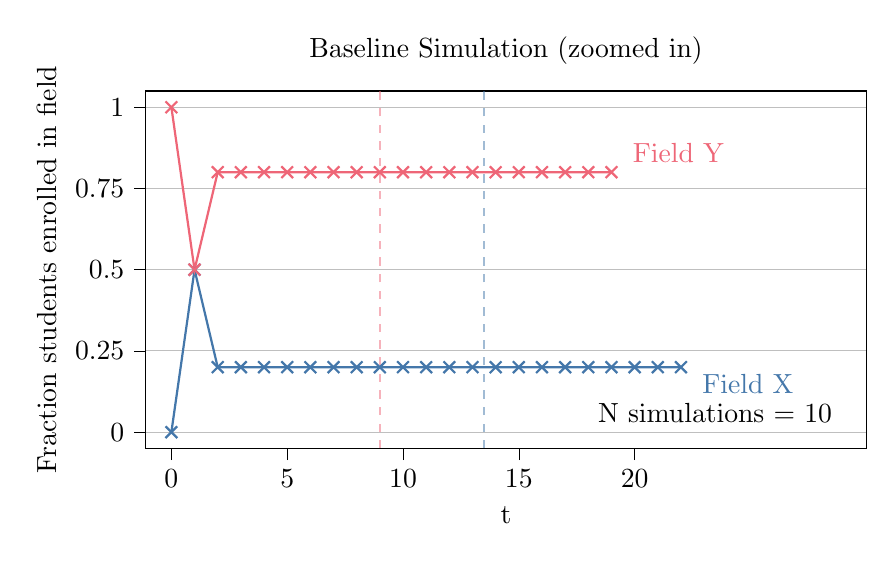
\begin{tikzpicture}

\definecolor{color0}{rgb}{0.266666666666667,0.466666666666667,0.666666666666667}
\definecolor{color1}{rgb}{0.933333333333333,0.4,0.466666666666667}

\begin{axis}[
height=6.121302808757603cm,
tick align=outside,
tick pos=left,
title={Baseline Simulation (zoomed in)},
unbounded coords=jump,
width=10.729849cm,
x grid style={white!69.0196078431373!black},
xlabel={t},
xmin=-1.1, xmax=30,
xtick style={color=black},
xtick={0,5,10,15,20},
xticklabels={
  \(\displaystyle 0\),
  \(\displaystyle 5\),
  \(\displaystyle 10\),
  \(\displaystyle 15\),
  \(\displaystyle 20\)
},
ylabel={Fraction students enrolled in field},
ymajorgrids,
ymin=-0.05, ymax=1.05,
ytick style={color=black},
ytick={0,0.25,0.5,0.75,1},
yticklabels={
  \(\displaystyle 0\),
  \(\displaystyle 0.25\),
  \(\displaystyle 0.5\),
  \(\displaystyle 0.75\),
  \(\displaystyle 1\)
}
]
\addplot [thick, color0, mark=x, mark size=3, mark options={solid}]
table {%
0 0
1 0.5
2 0.2
3 0.2
4 0.2
5 0.2
6 0.2
7 0.2
8 0.2
9 0.2
10 0.2
11 0.2
12 0.2
13 0.2
14 0.2
15 0.2
16 0.2
17 0.2
18 0.2
19 0.2
20 0.2
21 0.2
22 0.2
};
\addplot [thick, color1, mark=x, mark size=3, mark options={solid}]
table {%
0 1
1 0.5
2 0.8
3 0.8
4 0.8
5 0.8
6 0.8
7 0.8
8 0.8
9 0.8
10 0.8
11 0.8
12 0.8
13 0.8
14 0.8
15 0.8
16 0.8
17 0.8
18 0.8
19 0.8
20 nan
21 nan
22 nan
};
\addplot [semithick, color0, opacity=0.5, dashed]
table {%
13.5 -0.05
13.5 1.05
};
\addplot [semithick, color1, opacity=0.5, dashed]
table {%
9 -0.05
9 1.05
};
\draw (axis cs:22.5,0.12) node[
  anchor=base west,
  text=color0,
  rotate=0.0
]{Field X};
\draw (axis cs:19.5,0.83) node[
  anchor=base west,
  text=color1,
  rotate=0.0
]{Field Y};
\draw (axis cs:18,0.03) node[
  anchor=base west,
  text=black,
  rotate=0.0
]{N simulations = 10};
\end{axis}

\end{tikzpicture}
